\begin{figure}
 \centering
 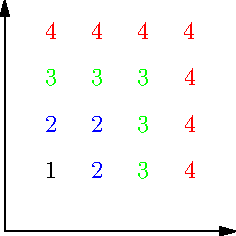
\includegraphics{./Ccu25_1.pdf}
 % Ccu25_1.pdf: 0x0 pixel, 300dpi, 0.00x0.00 cm, bb=
 \caption{Exercice \theenumi. \; $\max(i,j)$ \tiny{ (Ccu25)}}
 \label{fig:Ccu25_1}
\end{figure}

\begin{tiny}(Ccu25)\end{tiny} Calcul de $S$.
\begin{multline*}
 S = \sum_{i=1}^n \left( \sum_{j=1}^n i + \sum_{j=1}^n j\right) 
 = \sum_{i=1}^n \left( n i + \frac{1}{2}n(n+1)\right) \\
 = n^2(n+1)
\end{multline*}

Pour le calcul de $M$, on s'appuie sur le schéma des valeurs (figure \ref{fig:Ccu25_1}) qui permet de regrouper les valeurs égales.
\begin{displaymath}
 M =
 \sum_{k=1}^2(2k-1)k
\end{displaymath}
On écrit $2k-1=2(k-1)+1$ d'où
\begin{multline*}
 M = 
2\sum_{k=1}^{n}k(k-1) +\frac{1}{2}n(n+1) \\
= \frac{2}{3}\sum_{k=1}^n\left( (k+1)k(k-1) - k(k-1)(k-2)\right) \\
+ \frac{1}{2}n(n+1)\\
= \frac{2}{3}(n+1)n(n-1) + \frac{1}{2}n(n+1)
= \frac{1}{6}n(n+1)(4n-1)
\end{multline*}

Comme
\begin{align*}
 \max(a,b) + \min(a,b) &= a+b\\
 \max(a,b) - \min(a,b) &= |a-b|
\end{align*}
On calcule $m$ et $a$ avec les relations
\begin{displaymath}
 m + M = S,\hspace{0.5cm} M - m = a.
\end{displaymath}

